% Preamble
\documentclass{aastex631}

% imported packages
\usepackage{graphicx}

% reset commands to set the line spacing
\renewcommand{\baselinestretch}{1.5}

\begin{document}

\title{The Temporal Evolution of the Tidal Disruption Event AT2024wsd}

\author[0000-0003-4537-3575]{Noah Franz}
\affiliation{Department of Astronomy \& Steward Observatory, University of Arizona}

\begin{abstract}
  This is an abstract
\end{abstract}

\section{Introduction}

\section{Methods}
\subsection{Kuiper 61'' Observations}
\subsection{Data Calibration}

\subsection{Signal Extraction and Flux Calibration}

\begin{figure}
  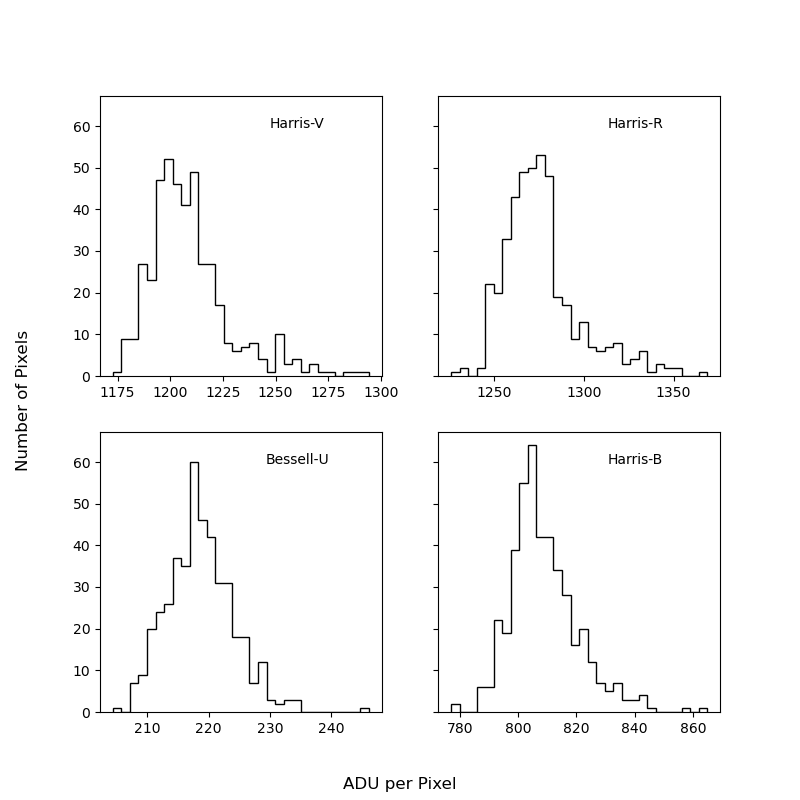
\includegraphics[width=\textwidth]{../analysis/aperture-counts-hist.png}
  \caption{Caption}
  \label{fig:aperture-counts}
\end{figure}

\begin{figure}
  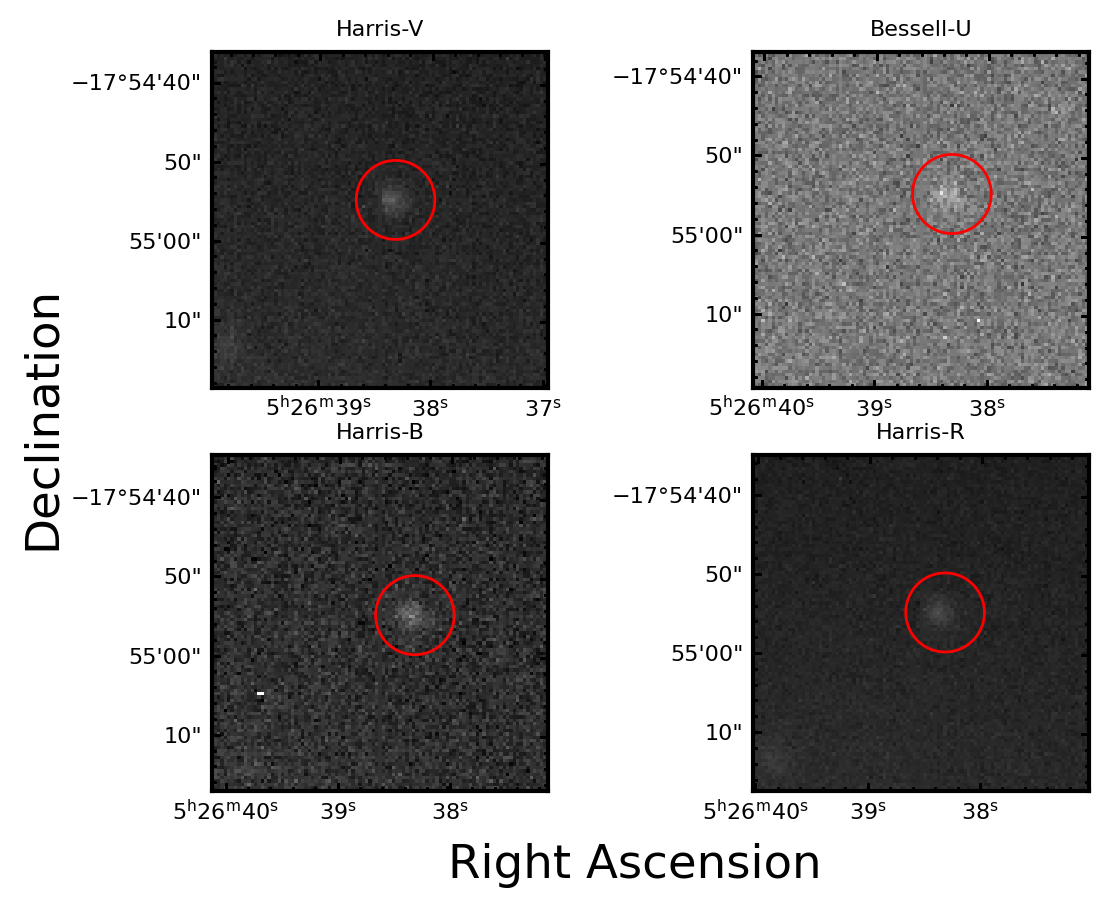
\includegraphics[width=\textwidth]{../analysis/target-images.png}
  \caption{Caption}
  \label{fig:targ}
\end{figure}

% \begin{figure}
%   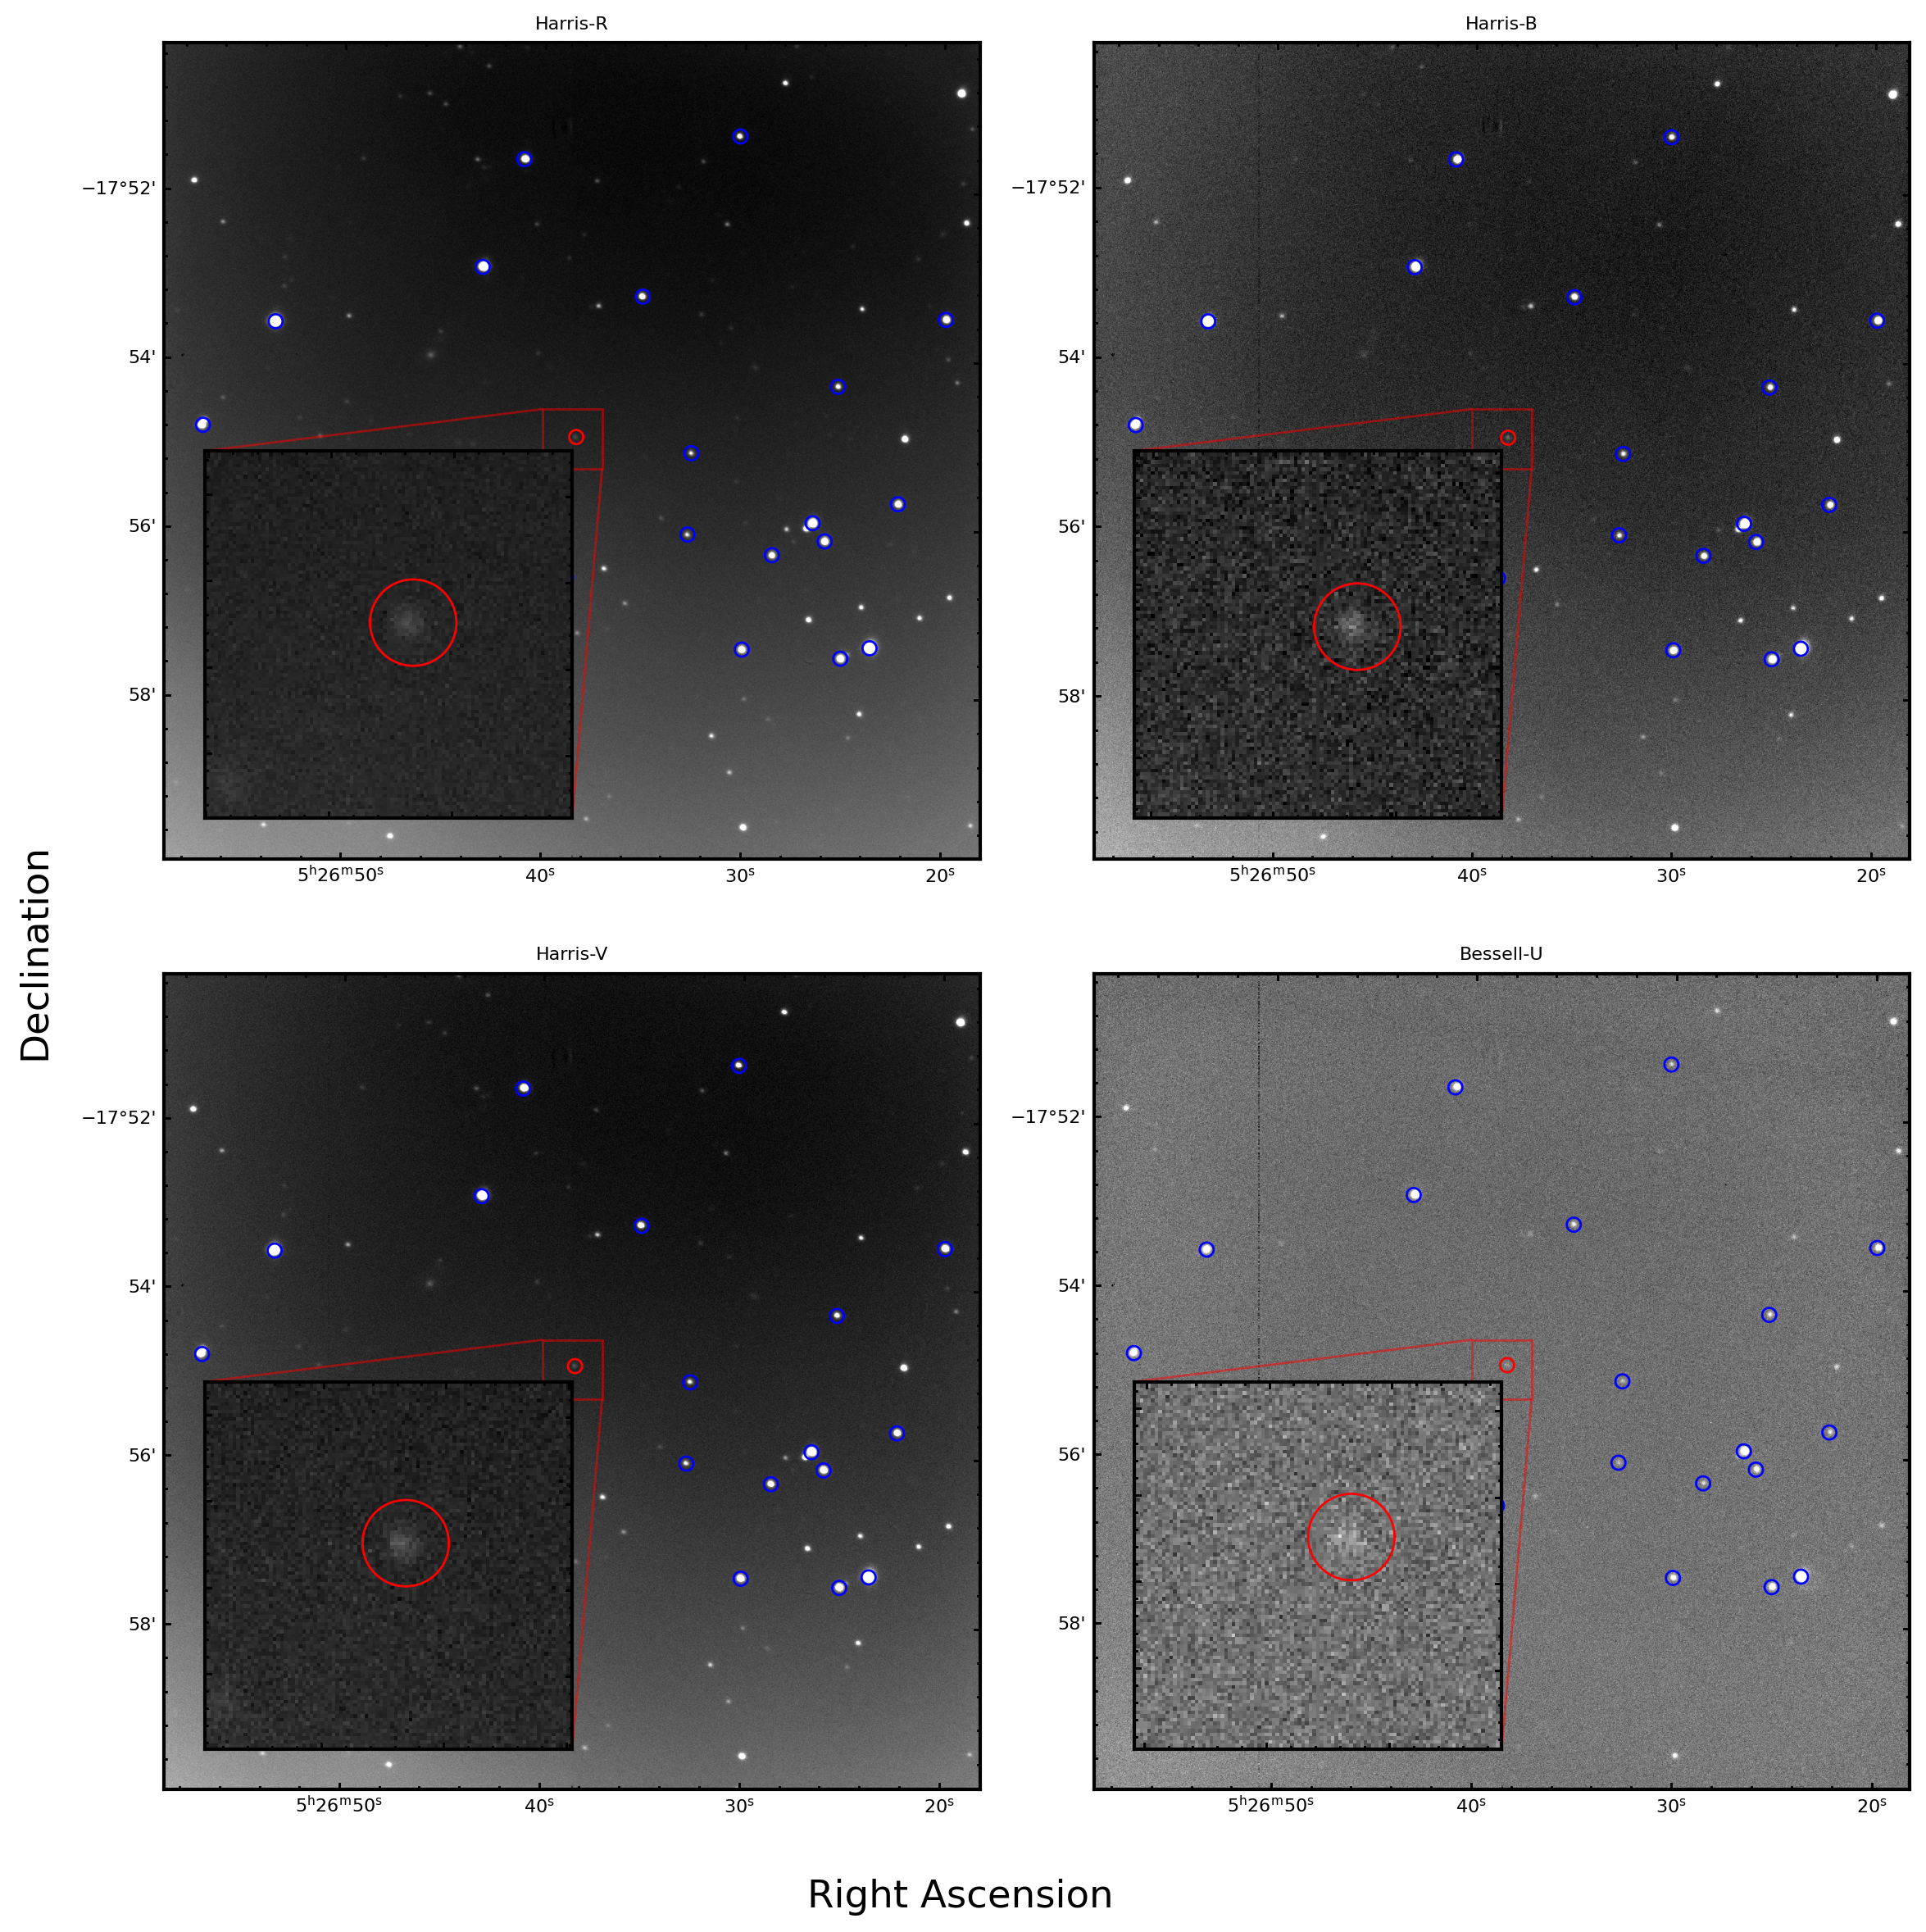
\includegraphics[width=\textwidth]{../analysis/fcal-images.png}
%   \caption{Caption}
%   \label{fig:fcal}
% \end{figure}

\subsection{SED Modeling}

\section{Results}
\subsection{Observational Results}

\begin{table}
\caption{Reduction Results}
\label{tab:res}
\begin{tabular}{lllll}
Filter & Harris-V & Bessell-U & Harris-B & Harris-R \\
Source Aperture Sum (ADU) & 525131.38 & 95118.46 & 352222.45 & 554880.18 \\
Source Aperture Sum (e) & 1627907.28 & 294867.23 & 1091889.60 & 1720128.57 \\
Source Aperture Sum ($\gamma$) & 2711100.28 & 491068.91 & 1818421.88 & 2864684.69 \\
Background Annulus Sum (ADU) & 521430.41 & 94325.44 & 348674.99 & 549048.02 \\
Background Annulus Sum (e) & 1616434.28 & 292408.86 & 1080892.45 & 1702048.85 \\
Background Annulus Sum ($\gamma$) & 2691993.26 & 486974.75 & 1800107.34 & 2834574.90 \\
Dark Noise ($\sigma_D$; ADU) & 0.29 & 0.29 & 0.29 & 0.29 \\
Dark Noise ($\sigma_D$; e) & 0.51 & 0.51 & 0.51 & 0.51 \\
Read Noise ($\sigma_R$; ADU) & 3.26 & 3.26 & 3.26 & 3.26 \\
Read Noise ($\sigma_R$; e) & 10.10 & 10.10 & 10.10 & 10.10 \\
Signal ($f_e$; e) & 11473.00 & 2458.37 & 10997.15 & 18079.72 \\
Signal ($f_\gamma$; $\gamma$) & 19107.02 & 4094.15 & 18314.54 & 30109.79 \\
SNR & 8.74 & 3.94 & 10.10 & 13.42 \\
Zero Point ($10^{12}f_0$; $\gamma$) & 0.47 & 0.05 & 0.33 & 0.44 \\
Apparent Magnitude & 18.48 & 17.72 & 18.14 & 17.92 \\
Apparent Magnitude Error & 2.11 & 4.49 & 1.80 & 1.34 \\
\end{tabular}
\end{table}


This is where things like SNR and extracted magnitudes will go

\subsection{Modeling Results}

\section{Conclusions}

\end{document}

%%% Local Variables:
%%% mode: LaTeX
%%% TeX-master: t
%%% End:
